\documentclass[10pt,a4paper]{article}
\usepackage[latin1]{inputenc}
\usepackage{amsmath}
\usepackage{amsfonts}
\usepackage{amssymb}
\usepackage{hyperref}
\usepackage{parskip}
\usepackage[subrefformat=parens]{subcaption}
\usepackage{pgfplots}
\pgfplotsset{compat=1.16}
\usepackage{sidecap}
\usepackage[left=2cm,right=2cm,top=2cm,bottom=2cm]{geometry}
\author{Samuel Russell}
\title{Innocuous Ciphertexts}
\begin{document}
\maketitle

\section{Contributions}

\begin{itemize}
\item Critically discuss the downfalls of using an FTE system to encode ciphertexts.
\item Build a statistical tool for distinguishing emulated from normal traffic.
\item Build a new scheme that is able to overcome this detection.
\end{itemize}

\pagebreak
\section{Introduction}

\pagebreak
\section{Motivation}

Tim Berners-Lee says\cite{gard} that since its conception, the world wide web has been built with the principles of openness and privacy. These key values, that also lie at the heart of democracy, can ensure that if a website is made available on web, anyone can connect to it - no matter who they are or where they live. 

However, recently, changes have been made which challenge this status quo. These changes are the censorship of certain content on the internet for users in some places like the United Kingdom or in China. The motivations behind this censorship can be well-meaning, for example, the blocking of illegal content such as child pornography with the intention of protecting the innocent lives of children. Further attempts to reduce damage to people's lives was the implementation of search engine de-listing of personal content partitioned by the right-to-be-forgotten movement\cite{rtbf}. This decision sparked much controversy since people believed that this deletion of history could lower the quality of the internet. 

However, other cases are on a much larger scale, such as nation states blocking access to content that they deem to be opposing to their political standpoints. This can involve blanket restrictions to foreign websites or restricting sites, which may be hosted inside the nation, but are deemed to perpetuate negative views. Many countries ban hate-speech, or exclude it from their freedom of speech laws\cite{hate} and some countries have Libel rules\cite{libel} which ban spreading of false information. However, there are a number of nations that actually hide information about certain world events or ideologies from their citizens, depriving their civil rights\cite{chincensor}. This is dangerous for the world as it creates environments that can breed hate directed at whomever the censors want.

There is no doubt that the western economy and society has benefited greatly with the success of the web with its ability to connect people and share information. What ensures the web's success is it's status as a permissionless space that leads to creativity, innovation and freedom of expression. This allows any new, small, start-up companies and individuals to use this commodity to build services and communities without the need for legal approval or business deals, leaving their projects to be free to grow and prosper. Proposed Net Neutrality regulations would have allowed internet service providers to prioritise certain site's traffic. This does not permit full censorship but even the slowing down of traffic could reduce the usability of certain sites so that users would avoid them. This would fundamentally coerce browser's behaviour to direct them away from certain topics.

Taking an existing example; in China, which is a state with among the most stringent internet censorship practices, the American Chamber of Commerce\cite{amcham} says that 4 out of 5 of its member companies report a negative impact on their business from Internet censorship. This gives financial incentives to ensure the internet remains open.

\section{Network Surveillance and Censorship}

I will categorise censorship in two ways. The first kind is entities on the internet such as websites taking down content. This is most poignant when the content has been made by others, such as on a micro-blogging site like Facebook. Although, this is an issue and currently there is debate about the balance of such censorship on these social media platforms, this is not what I will be looking at. This is because the data is gone rather that being blocked. Of course, there are tools that archive content that maybe be later re-tracked or deleted such as The Internet Archive's project: Wayback Machine\cite{wb}, and access to these resources is what the second type of censorship is about.

The internet consists of each party's computer equipment connected together with a network of wires (and other mediums) and some management machinery to route communications to their destination.  Communications are packet based and are directed along the connections according to the Internet Protocol (IP)\cite{ip4}. This protocol defines the destination of the packet for the purposes of working out the most appropriate route to follow. It also contains the address of the source so error messages can be directed appropriately. Among other information like version numbers and flags there is also a field that tells the intermediary machinery when to delete the message, but this is only for cases where the destination in unreachable. 

The second type of network surveillance and censorship sits at these intermediate points in the network and deals with how these packets are handled. By default IP and the transport layer on top of it (TCP) does not encrypt or sign the payload data. Therefore, it is possible for the intermediary parties to read and tamper with the packets and their payloads before they are sent or even dropped from the network. 

From their observations of the chinese internet filtering systems, Zittrain and Edelman\cite{edelman2005empirical} deduced several methods that were being used. Filtering on the IP address of a resource can be done by analysing the destination field of the packet. This is good for blocking direct access to static sites since it  is one of the simplest and therefore fastest to implement, though it relies on comprehensive black listing coordination.

The most common method of blocking is for the routers to drop these packets, but as Clayton et al. found in their practical experiments\cite{clayton2006ignoring} for protocols that communicate in a streaming fashion over time the network machinery sends TCP reset packets to both parties to interrupt the session and stop communication. This type of attack can be easily countered by ignoring all reset packets since due to how the system is architectured the original packets are allowed through. They also observed a less frequent technique which was the injection of a forged packet with random synchronisation numbers. When this reaches the destination the server detects the incorrect value and validly triggers the reset packet. Now, if the reset packets are ignored then the two real endpoints become out of sync and the communication breaks down. Luckily as it stands, the forged packets are poor imitations and so are easily detectable.

Other method used in practice is DNS poisoning, which breaks involves incorrectly resolving URLs for users to redirect them to a Censorship notice or just a random useless address. This only affects the use of URLs and so raw IP address access is completely unaffected, although many sites use them internally so it creates great difficulty and work for users.

Finally, packet inspection has become very common place. This can be content based detection such as searching for trigger words in HTTP request paths, or in the html content returned. A good example of this is search terms in search engine requests. Although this only applies to clear unencrypted http traffic and using an encrypted  TLS transport layer hides all this information sites that use this risk having the whole site IP blocked as above. This happened to Wikipedia in China when the site switched to enforcing HTTPS on all traffic.

The packet inspection is also done on a protocol basis. Censors are usually tolerant to users accessing webpages over HTTP or video calling over VOIP protocols, however, protocols that allow the transfer of data in a opaque way such as VPN tunnelling, The Onion Router and in general TLS are often blocked completely.

\section{The Onion Router}

One of the most effective tools for evading network surveillance is The Onion Router which not only hides the contents of packets like TLS, but also obfuscates their destination. It does this by maintaining a opaque network which decorrelates the inputs and outputs. Therefore, it is hard to workout where traffic that enters the network at an entry node will exit, and then therefore what its final destination is. To realise this, each packet is encrypted 3 times (on top of standard TLS encryption) and, as the packet moves through the network, a layer of encryption is removed at each relay node. This means, as it mixes with other packets it is hard to identify. Paths through the network are randomly allocated and keys are exchanged securely using a Diffe-Helman protocol. This is done one node at a time, through the existing link such that nodes only know the identities of their predecessor and successor in the chain. 

However, there has been a lot of work and success in to de-anonymising the TOR protocol to gather information on users. There has been research in to both passive and active attacks attacks giving varying levels of success but with varying levels of effort.  Website fingerprinting attacks such as Cair et al.\cite{webfinger} only need single point of eavesdropping but suffer from high false positives. Traffic confirmation attacks which require access to both ends of the cummunication such as Shmatikov et al.\cite{conf} need long periods to gain statistical significance. Active attacks such as water marking through delays are a lot quicker but they involve a lot more work for the attacker. However, government bodies with large powers such as the NSA are interested in this field so it is not out of the realms of possibility. Even so, if an adversary only controls a small proportion of the network the chances of being allocated a fully comprised relay chain is small. Recently, Arp et a.\cite{torben} released a side-channel attack for TOR which is more reliable but less intrusive that other methods that use browser exploits. In fact in their research Nithyanand et al.\cite{AS} found that very high levels of all circuits were potentially vulnerable to state level adversaries. To counter this, they have built a TOR client that is aware of adversaries and is able to more intelligently select relay paths. This is successful in reducing the rate of affected connections but as with all these techniques sacrifices performance, adding latency to the circuit generation before any data can be sent.

Although TOR has these issues, it makes the surveillance of users browsing astronomically harder and so censors such as the Chinese Government have resorted to a complete ban on the service. Tor packets are very recognisable due to their predictable size and structure but some improvement have been made to adjust it's fingerprint to match TLS as much as possible. 

Tor works by allowing users to connect to one of the publicly known entry guard relays however, since these IP addresses are public they are easily detected and interfered with by in-line systems. One way this is done is by sending reset packets to both parties telling them to close the TCP stream.
To circumvent this, users instead connect to private bridges in uncensored zones (such as the US) so that the indented destination of the packets was hidden. However, with protocol fingerprinting by deep packet inspection (DPI) and the use of active probes censors can still catch these unlisted bridges in under 15 minutes of use!
The use of FTE bridges has been able to fool these DPI systems for now since they fool the common protocol classification systems which use regular expressions also. However, as deep learning becomes more prevalent it is known that this will not be enough.


\pagebreak
\section{Cryptography Background}
After language was invented to share knowledge, humans soon needed a way hide it from those whom it was not intended. The first schemes used word or letter substitutions or the shuffling of characters to make the meaning of a message hard to obtain. These techniques are still used as the basic building blocks today; for example in the AES block cipher, a very popular encryption scheme, of which there are hardware implementations baked in to many of the major computer chips. Early schemes however, relied on the secrecy of the method to protect the privacy of the message which meant that they cannot be reused by others. This lead to the introduction of parametrised constructions that use a key to alter the encryption such as the Vigen\`ere cipher. Modern schemes obey Kerkoff's principle; that the security of the system only depends on the security of the key, allowing the same encryption method to be used by all.
\begin{itemize}
 \item security through obscurity
 \item perfect security - information-theoretic
 \item conditional security
 \item ciphertexts - formatting
 \item block ciphers
\end{itemize}

\begin{itemize}
 \item hiding existence
 \item stenography
 \item honey encryption
 \item deniable encryption
\end{itemize}

\pagebreak
\section{Format Preserving Encryption}

In 1981, NIST\cite{FIPS74} outlined a mode of DES that was able to restrict the ciphertext of an encryption to a string of a fixed, finite alphabet such as decimal digits $ \Sigma = \{0,1...9\} $. This allows plain texts such as phone numbers of form $ X \in \Sigma^N $ to be encrypted to a ciphertext $ Y = \Sigma^N $ that is also a phone number. Although that FIPS document is now withdrawn it sparked further work such as Brightwell and Smith\cite{DPE}. They first specify the particular use case of encrypting data in place in a database where the ciphertexts must abide by the same type constraints of the database schema. The paper then goes on to describe their  Datatype-Preserving Encryption scheme that again works with DES in a streaming mode and works over an indexed finite alphabet, however the algorithm has redundant elements such as shuffling the alphabet's ordering that are not backed up with reasoning and there is no proof of security. More recently, Black and Rogaway\cite{CAFD} provide three constructions in their paper. They analyse the security of each one against the standard adversary $Adv^{prp}$ and also discuss the practical considerations of scaling.

The field has become a highly practical one, with companies such as Voltage moving to take advantage of the concept. They are using it to upgrade older systems by adding a layer of security that since does not change the structure of the data is invisible to the applications that sit on top. Therefore the costs of this retrofitting is vastly reduced since the need to completely redesign the system is usually eliminated. As of 2018, HPE\cite{hp} are still pushing it as part of their SecureData product to help maintain legacy software.

To keep up with the work in industry, Bellare et al. wrote a comprehensive paper\cite{fpe} that formally defines the goals of FTE. They did this in the form of adversary based games. They redefine the standard Pseudo Random Permutation (PRP) Security game which challenges an adversary to distinguish the encryption scheme from a random permutation. The paper also gives weaker notions they think are more appropriate. Single Point Indistinguishably (SPI) requires the adversary to be unable to distinguish between the encryption of any chosen plaintext and a randomly selected ciphertext. The Message Recovery (MR) game gives the adversary the distribution of plaintexts and asks for a decryption of a randomly selected ciphertext, given an encryption and verification oracle. Finally they define Message Privacy (MP) as the inability of an adversary to compute a function of a plaintext given the ciphertext; Note in this game the adversary can select the function it hopes it will have most success with. They state the following strength hierarchy for these games, showing PRP does give us the Message Recovery property we ultimately want.
$$ PRP \implies SPI \implies MP \implies MR $$
The first implication is trivial since a random function will produce a random element when given the message. The last last implications is also trivial since MR is just a special cast of MP - where the function is fixed to be the identity. For the proof of $ SPI \implies MP $ the paper shows how an adversary $B$ for SPI can be  constructed using an adversary $A$ for MP with sufficiently large advantage since $B$ is able to run $A$ and satisfy it's calls to the encryption oracle using its own oracle.

\subsection{Rank and Encrypt}

In the second half of the paper\cite{fpe} Bellare et al. then proposed a framework called Rank then Encipher. This framework supports and enhances the methods already discussed since it enables any encryption scheme that supports arbitrary size alphabets to be used to encrypt more complex languages. It simplifies the complexity of language features such as a checksum character by maps words to an simple index so that the encryption scheme used can be generic. It does this by partitioning the language in to slices of the words of each length. That is, for the language $\mathcal{X} = \{\mathcal{X}_N : N \in \mathcal{N} \}$ for lengths $\mathcal{N}$, each slice $\mathcal{X}_N = \{ X : X \in \mathcal{X}, \vert X \vert = N  \}$. Now each slice can be arbitrarily ordered as $\mathcal{X} = \{ X_0, X_1, \cdots , X_{n-1} \} $ and a bijective mapping can be defined $rank_N :: \mathcal{X}_N \rightarrow \mathbb{Z}_n$.
Then for the whole language, we can define
$$ rank :: \mathcal{N} \times \mathcal{X} \rightarrow \mathbb{N} \cup \bot $$
$$ rank(N,X) =
\left\{
	\begin{array}{ll}
		rank_N(X)  & \mbox{if } \vert X \vert = N\\
		\bot & \mbox{otherwise} 
	\end{array}
\right.
$$

$$ unrank :: \mathcal{N} \times \mathbb{N} \rightarrow \mathcal{X} \cup \bot $$
$$ unrank(N,i) =
\left\{
	\begin{array}{ll}
		rank_N^{-1}(i)  & \mbox{if } i \in \mathbb{Z}_{\mathcal{X}_N}\\
		\bot & \mbox{otherwise} 
	\end{array}
\right.
$$

Then if we have an encryption scheme $Enc :: \mathcal{K} \times \mathcal{N} \times \mathbb{N} \rightarrow \mathbb{N}$ that works over arbitrary domains to encrypt values into $\mathbb{Z}_{|\mathcal{X}_N|}$, we can define out scheme $\mathcal{E}_k^N = unrank_N \cdot Enc_k^{|X_N|} \cdot rank_N$. Using this construction, they state how the security properties of the original encryption scheme over the finite domain is inherited by the the rank then encrypt scheme over the language.

They provide a ranking and un-ranking algorithm for regular languages, but to make this efficient, pre-computation is needed. For each word length a table has to be created which can be done through dynamic programming.

Furthermore, using M\"akinen's\cite{rankcf}, algorithms if a language can be described an unambiguous context free grammar then ranking can be done in linear time and unranking can be done in $O(n \log n)$ time, if we allow $O(n^2)$ time and space preprocessing. This is since the left Szilard language of the grammar can be more easily ranked and unranked. Conversion back to the original grammar is as simple as linearly applying the rules and conversion from a word to it's left Szilard counterpart depends on the efficiency of parsing, which, is not linear, but for unambiguous grammars is still efficient.

\section{Format Transforming Encryption}

Inspired by the rank and encrypt method from Bellare, Dyer et al. outlined in their paper\cite{fte} a new cryptographic primitive that extends standard symmetric encryption to produce ciphertexts that follow a selected format. This is done by chopping the front off the the scheme $\mathcal{E}^N_k$ defined above and interpreting the input bit stream as a number that represents the ranking.

Their scheme is targeted against the regular expression based deep packet inspection (DPI) schemes that are commonly used in industry. These high end DPI tools are deployed by network administrators all over the world as they are able to label traffic by protocol using the regular expressions as definitions. They are attractive because they are fast, due to the speed of finite state machine automatons and can single out suspect type of traffic for further analysis of payloads.

They show in their paper that FTE leaves these systems vulnerable to protocol misclassification by targeting allowed formats that can either be extracted from the enterprise software or learned by taking network samples. They also show that the formatting encryption expansion factor for realistic regular expressions is low enough to enable web surfing over the TOR protocol.

Formally, the scheme takes a formatting regular expression grammar $\mathcal{F}$ and lets $L(\mathcal{F})$ be the language defined by it. Then using an existing authenticated encryption scheme $Enc_k$ encrypts the original message $M$ and interprets the unformatted ciphertext $Y$ as an element of $\mathbb{Z}_{\vert L(\mathcal{F}) \vert}$. The encoding function $unrank :: \mathbb{Z}_{\vert L(\mathcal{F}) \vert} \rightarrow L(\mathcal{F})$ is then used to format it to specification. To make \texttt{unrank} and it's inverse, decryption counterpart \texttt{rank} efficient the same precomputation is done as by Bellare and only a subset of the formatted language with fixed length is used. This turns the use of the scheme in to a block cipher used in Electronic Code Book mode. However, this lack of diffusion does not lead to pattern leakage since a random IV is used for each large block.

They have integrated their scheme in to a TOR transport and they have had success in bypassing China's Golden Shield Project (GSP) censorship mechanisms.

%https://blog.torproject.org/iran-partially-blocks-encrypted-network-traffic

%Instead must use advanced mechanisms (discussed in Section 7) in settings with adversarial users.

\pagebreak
\section{Distribution Transforming Encryption}

Although FTE produces validly formatted ciphertexts which satisfies many current filtering systems, the ciphertexts look in no way normal, such in the way that auto generated C source code looks very different to any C code that a human would write. This means that statistical analysis will discover that these streams are in fact fake. My scheme will try and form ciphertexts that are comparable to a stream of normal browser HTTP traffic.

To do this, there must be a way to encapsulate not just the valid language but its frequency distribution. Sadly, augmenting the finite state machine produced by the regular expression with weights does not produce the desired effect. Adding weights to the DFA's state transitions would still produce a graph that could be ranked using a slightly altered algorith. However, these weights would not be meaningful, since they would not be taking in to consideration the previous path through transition graph and therefore previous symbols in the stream. In some graphs, where every different input stream parses through a different subset of the DFA states this approach is valid. However, efficient DFA's do not do this since it has exponential blow up.

In fact, however you encode it, to fully define the probability density function for a bit stream of even a fixed length $n$, you also need exponential space. For example let's calculate the space requirement for a block of payload of size $10$ bytes long. Assume a 4 byte fixed point or floating point value is used to store the proportions, depending on the variation of the values. The storage size would be an intractable $4*(256^10) = 4*(1024^8) = 4$ yobi bytes.

Therefore, obviously simpler distribution descriptions were needed i.e. heuristics. The first target is to design a distinguisher for the existing FTE scheme from normal traffic. The first heuristic was targeted at the fixed width that Dyer scheme produces. It can be clearly seen in figure \ref{fig:fake_length_dist} that compared to normal traffic the difference is obvious.

\begin{figure}[h]
\begin{subfigure}[b]{.49\linewidth}
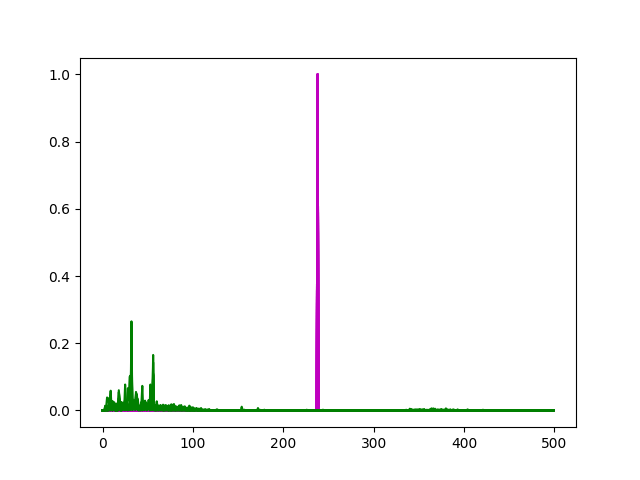
\includegraphics[width=\linewidth]{fake_length_dist}
\caption{Normal vs. FTE fixed width}
\label{fig:fake_length_dist}
\end{subfigure}
\begin{subfigure}[b]{.49\linewidth}
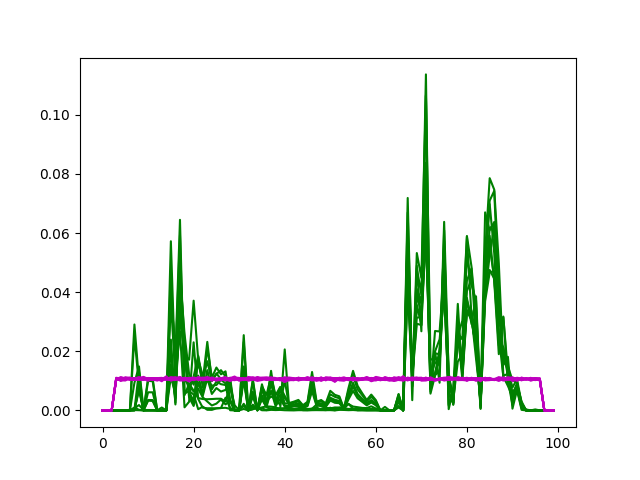
\includegraphics[width=\linewidth]{uniform_length_dist}
\caption{Normal vs. random width}
\label{fig:uniform_length_dist}
\end{subfigure}
\caption{Length Distrbutions}
\end{figure}

In this case, the probability of the packet being exactly 256 bytes is overwhelmingly greater for the FTE scheme than form normal traffic. Of course, legitimate packets may also be this length so filtering them all out would give false positives. This might be okay if when the TCP layer resent the data it would be different as so would be let through but it sends an exact copy each time. Therefore, to amplify the probability of not catching false positives, then system must take a sample from the stream and check them all. This could be done on a small running window basis and when triggered will add the IP address to a temporary ban. This is like what happens in currently deployed keyword filtering systems such as in China. 

Another heuristic for defining the distribution is pattern frequency. This can be done at varying levels of granularity. 

\pagebreak
\section{Implementation}


I have implemented the code for the censor and the de-censor scheme. The censor implementation consists of a measurement program that calculates the statistical similarity of batches of paths to a pre-recorded reference histogram of normal traffic. It compares the statistic to a threshold pre-calculated to separate normal from malicious requests. The de-censor scheme takes in messages, encrypts them and then encodes them using the selected emulator, that outputs an expanded ciphertext but one that is distributed according to it's reference histogram. This can be the same reference distribution as the censor, but a high success rate is also possible using a separately recorded histogram of the same normally distributed background traffic. This is important since practically, it would not be possible to extract the used distribution from in-use instances of the tool.


All the code was written in \texttt{python2.7} for quick prototyping but for performance gains the core could be re-written in \texttt{C/C++} to remove the overheads of the python interpreter. I conducted my implementation and testing on Ubuntu 16.04 on VMware virtual machines running on a low powered i5 Intel VT enabled laptop.

\subsection{Collection}

Packet collection is used for both parties, since both the emulator and censor need to record a reference distribution to work against and the censor is also required to read the packets for classification. Since both my censor and de-censors are running on Ubuntu machines I used the PyShark a python wrapper around the Tshark non-interactive command-line tool. Tshark is also able to parse and filter the packets like currently deployed DPI systems. I used this feature to extract the packets I cared about using the filter in figure \ref{fig:filter}.

\begin{figure}[h]
\begin{verbatim}
http && http.request.method == "GET"
\end{verbatim}
\caption{Tshark packet filter}
\label{fig:filter}
\end{figure}

The filter shows that we only targeted GET requests. This is because HTTP is a very one sided protocol with most of the content moving from the web server to the client and therefore it is harder to hide messages inside the requests. The response encoding should be more straight forward. GET requests as opposed to POST requests take up a larger proportion of web traffic and so are the obvious choice. 

In this experiment I have fixed all other parameters apart from path. This is a proof of principle
of the sides of communication to forge due to it's normally low data size. Files returned from servers are usually much less structured 

To collect real web traffic data, I built a web-crawler using the FOSS Selenium web automation framework. To gather a realistic distribution I needed to emulate the whole browser environment since X amount of the requests from modern sites are dynamics initiated from inside the scripts.
% graph

I crawled recursively over the Alexa top 50 sites\cite{alexa} that support unencrypted traffic. This gave me a sample of 10,000 paths to create reference distribution.

\subsection{Histogram creation}

Like the recording of reference material, the calculation of distribution histograms is not time critical since they can be done offline. The process is straightforward frequency bins to count the occurrences of each option. I tried several methods as explained below.


\begin{figure}[h]
	\centering
	\begin{subfigure}[b]{0.24\textwidth}
		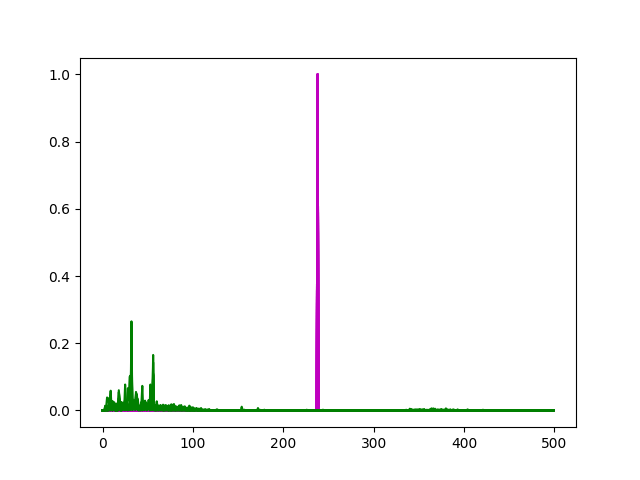
\includegraphics[width=\textwidth]{bob}
		\caption{Path length}
		\label{fig:length_hist}
	\end{subfigure}
	\begin{subfigure}[b]{0.24\textwidth}
		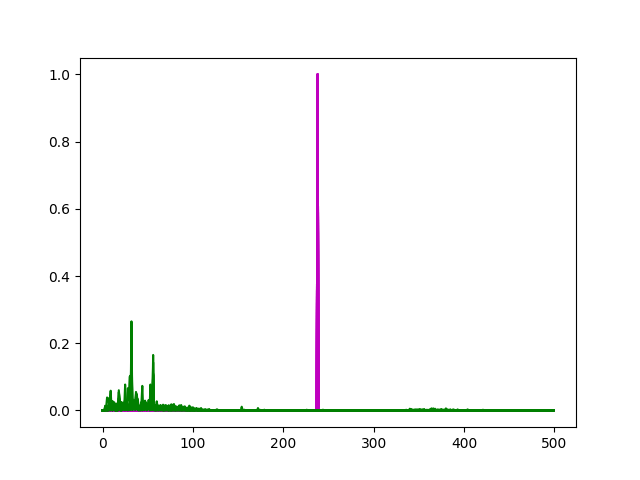
\includegraphics[width=\textwidth]{bob}
		\caption{Character based}
		\label{fig:char_hist}
	\end{subfigure}
	\begin{subfigure}[b]{0.24\textwidth}
		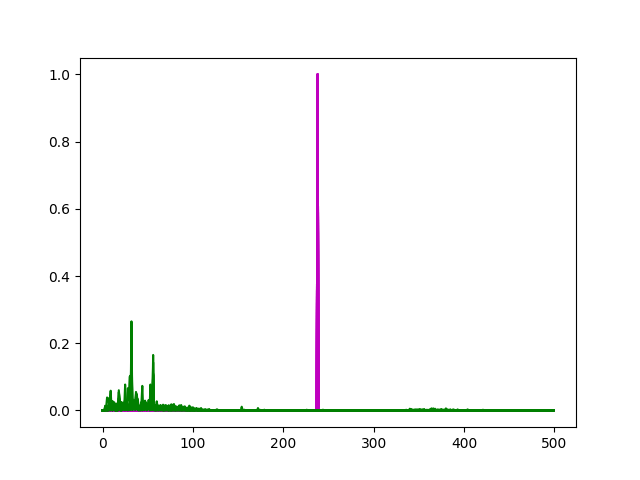
\includegraphics[width=\textwidth]{bob}
		\caption{First Letter}
		\label{fig:first_hist}
	\end{subfigure}
	\begin{subfigure}[b]{0.24\textwidth}
		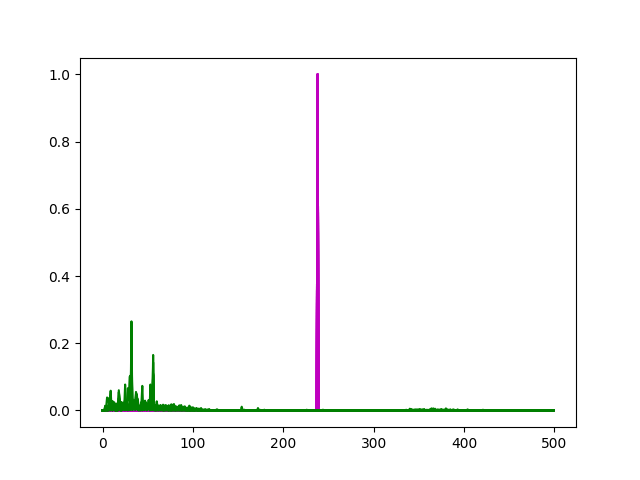
\includegraphics[width=\textwidth]{bob}
		\caption{Random Letter}
		\label{fig:rand_hist}
	\end{subfigure}

	\caption{Distribution Histographs}\label{fig:hists}
\end{figure}

Path length - this was targeted at the FTE scheme that used a fixed length. It shows very few examples would be needed to differentiate the origins.

Character distribution - This graph exibits the underlying encryption schemes uniform randomness, whereas in real traffic not all characters are created equally.

First Letter - This method was attempted to see if the same distinguishing effect would be possible only using a fixed subset of the URL.

Random Letter - like the previous this uses a limited sample by randomises it's location to see if this improved on the above results.


\begin{enumerate}
\item offline - so not performance critical
\item smoothing
\end{enumerate}

\subsection{Statistical Analysis}

\begin{enumerate}
\item finding good binning methods
\item Chi Square vs fischer test
\item thresholding, approximating to normal
\item library used
\end{enumerate}

\subsection{Encryption}

The DTE is an encrypt-then-encode framework. To ensure the same standards of encryption as in the FTE scheme DTE must also provide IND-CCA security. To ensure this I will use an authenticated encryption scheme i will use counter mode with HMAC using AES256 for encryption and SHA256 for authentication. Therefore, assuming the underlying block cipher - AES - is secure, this mode provides indistinguishability under a chosen ciphertext attack. This security guarantee is only for the encryption layer. 

%Now prove the property holds for the whole scheme

I used the Cryptography implementation from the PyCrypto library. This provides an AES block cipher, SHA256 Hash in a Merkle-Damg$\mathring{a}$rd construction and counter mode framework. The IV is chosen randomly.

\subsection{Proxy Embedding}

\pagebreak
\section{Evalutation}

\pagebreak
\section{Other Solutions}

ObfsProxy simply encrypts the entire packet with a streaming cipher. Earlier versions used a fixed parameters so although expensive, decryption could be done to obtain the standard traffic but now even that is not possible since a key exchange produces ephemeral keys. This procedure produces ciphertexts that are computationally indistinguishable from a random string so intensive computational statistics would be able to differentiate this from a background distribution of standard traffic. Also, do to it's complete lack of structure it would not pass any protocol white-listing filters.

StegoTorus is a system that uses carefully hand crafted embeddings for ciphertexts. In the HTTP mode, it selects randomly for pre-recorded traces and hides the chopped up ciphertext inside Javascript, PDF and SWF files and header fields like Cookies. Since, the masquerading protocol is HTTP, blocking encrypted protocols will not stop this. However, it relies on distributing large volumes of these traces or everyone recording their own, otherwise censors could just block all of them specifically. This means the overhead in communication but mainly storage of traces is large 


meek\\
Description: Is a transport that uses HTTP for carrying bytes and TLS for obfuscation. Traffic is relayed through a third-party server (Google App Engine). It uses a trick to talk to the third party so that it looks like it is talking to an unblocked server.

ScrambleSuit\\
Description: Is a pluggable transport that protects against follow-up probing attacks and is also capable of changing its network fingerprint (packet length distribution, inter-arrival times, etc.).
Language: Python

SkypeMorph\\
Description: It transforms Tor traffic flows so they look like Skype Video. See its source code and design paper.

Dust\\
Description: It aims to provide a packet-based (rather than connection-based) DPI-resistant protocol. See its git repository.


\pagebreak
\begingroup
\raggedright
\bibliography{thesis}{}
\bibliographystyle{plain}
\endgroup
\end{document}